% ------------------------------------------------------------------------
% ------------------------------------------------------------------------
% Modelo de trabalho acadêmico (Dissertações e Teses) do Programa de Pós-
% graduação em Física da Universidade Federal de Minas Gerais.
% Esse modelo é baseado na classe abntex2 (http://www.abntex.net.br)
% 
% ------------------------------------------------------------------------
% ------------------------------------------------------------------------

\documentclass[
	% -- opções da classe memoir --
	12pt,				% tamanho da fonte
	openright,			% capítulos começam em pág ímpar (insere página vazia caso preciso)
	twoside,			% para impressão em frente e verso. Oposto a oneside ---- Este comando ajusta automaticamente as margens
	a4paper,			% tamanho do papel. 
	english,			% idioma adicional para hifenização
%	french,				% idioma adicional para hifenização basta retirar o comentário para utilizar
%	spanish,			% idioma adicional para hifenização basta retirar o comentário para utilizar
	brazil				% o último idioma é o principal do documento
	]{abntex2}

% ---
% Pacotes básicos 
% ---
\usepackage{lmodern}			% Usa a fonte Latin Modern			
\usepackage[T1]{fontenc}			% Selecao de codigos de fonte.
\usepackage[utf8]{inputenc}		% Codificacao do documento (conversão automática dos acentos)
\usepackage{indentfirst}			% Indenta o primeiro parágrafo de cada seção.
\usepackage{color}				% Controle das cores
\usepackage{graphicx}			% Inclusão de gráficos
\usepackage{microtype} 			% para melhorias de justificação
\usepackage{relsize}				% usado para definir tamanho de fontes no sumário
% ---

% ---
% Pacotes úteis 
% ---
\usepackage[final]{pdfpages}		% Para incluir arquivos pdf externos
\usepackage{amsmath,amssymb,amsthm}	% Pacote para melhorar apresentação de fórmulas matemáticas, símbolos e teoremas, respectivamente	
\usepackage{pdflscape} 		% Pacote para adicionar páginas em formato paisagem
\usepackage{multirow}			% Permite criar céluas com várias colunas ou linhas em tabelas
\usepackage{adjustbox}			% Pacote para ajustar a largura e altura de objetos como tabelas
%\usepackage{imakeidx}			% Gera o índice
% ---

\usepackage{lipsum}	 % pacote usado para gerar os textos dos apêndices e anexos

% ---
% Pacotes de citações
% ---
\usepackage[brazilian,hyperpageref]{backref}	 % Inclui um link nas referências para a página onde o documento foi citado.
\usepackage{cite}
\usepackage[fixlanguage]{babelbib}
\selectbiblanguage{brazil}


% --- 
% CONFIGURAÇÕES DE PACOTES
% --- 

% ---
% Configurações do pacote backref
% Usado sem a opção hyperpageref de backref
\renewcommand{\backrefpagesname}{Citado na(s) página(s):~}
% Texto padrão antes do número das páginas
\renewcommand{\backref}{}
% Define os textos da citação
\renewcommand*{\backrefalt}[4]{
	\ifcase #1 %
		Nenhuma citação no texto.%
	\or
		Citado na página #2.%
	\else
		Citado #1 vezes nas páginas #2.%
	\fi}%
% ---

% ---
% Informações de dados para CAPA e FOLHA DE ROSTO
% ---
\titulo{Modelo para teses e dissertações do departamento de Física da UFMG}
\autor{Fulano de Tal}
\local{Belo Horizonte}
\data{2017}
\orientador{Beltrano da Silva}
\coorientador{Sicrano José}
\tipotrabalho{Tese (Doutorado)}
%\tipotrabalho{Dissertação (Mestrado)}
%\tipotrabalho{Projeto de Tese}
\preambulo{Tese apresentada ao Programa de Pós-Graduação em Física do Instituto de Ciências Exatas da Universidade Federal de Minas Gerais como requisito parcial para obtenção do título de Doutor em Ciências.}
%\preambulo{Dissertação apresentada ao Programa de Pós-Graduação em Física do Instituto de Ciências Exatas da Universidade Federal de Minas Gerais como requisito parcial para obtenção do título de Mestre em Ciências.}
%\preambulo{Projeto apresentado ao Programa de Pós-Graduação em Física do Instituto de Ciências Exatas da Universidade Federal de Minas Gerais como requisito parcial para qualificação no curso de Doutorado em Física.}
% ---



% ---
% Configurações de aparência do PDF final
% ---
% alterando o aspecto da cor azul
\definecolor{blue}{RGB}{41,5,195}

% informações do PDF
\makeatletter
\hypersetup{
     	%pagebackref=true,
		pdftitle={\@title}, 
		pdfauthor={\@author},
    	pdfsubject={\imprimirpreambulo},
	    pdfcreator={LaTeX with abnTeX2},
		pdfkeywords={abnt}{latex}{abntex}{abntex2}{trabalho acadêmico}, 
		colorlinks=false,       		% false: boxed links; true: colored links
    	linkcolor=blue,          	% color of internal links
    	citecolor=blue,        		% color of links to bibliography
    	filecolor=magenta,      		% color of file links
		urlcolor=blue,
		bookmarksdepth=4
}
\makeatother
% --- 

% --- 
% Espaçamentos entre linhas e parágrafos 
% --- 

% O tamanho do parágrafo é dado por:
\setlength{\parindent}{1.3cm}

% Controle do espaçamento entre um parágrafo e outro:
\setlength{\parskip}{0.2cm}  % tente também \onelineskip

% ---
% compila o indice, caso haja.
% ---
%\makeindex
% ---

% ----
% Início do documento
% ----
\begin{document}

% Seleciona o idioma do documento (conforme pacotes do babel)
%\selectlanguage{english}
\selectlanguage{brazil}

% Retira espaço extra obsoleto entre as frases.
\frenchspacing 

\include{tex/capa}
% ----------------------------------------------------------
% ELEMENTOS PRÉ-TEXTUAIS
% ----------------------------------------------------------
\pretextual

\centerline{\large UNIVERSIDADE FEDERAL DE MINAS GERAIS}
\centerline{\large PROGRAMA DE PÓS-GRADUAÇÃO EM FÍSICA}

\vspace{5cm}

\centerline{\large FULANO DE TAL}

\vspace{5.5cm}

\centerline{\Large Modelo para teses e dissertações do departamento de Física}
\centerline{\Large da UFMG}

\vspace{10cm}


\centerline{\large BELO HORIZONTE}
\centerline{\large 20XX}
\newpage


% ---
% Folha de rosto
% (o * indica que haverá a ficha bibliográfica e deverá ser usado para teses 
%   e dissertações. Para projetos, favor retirar o *)
% ---
\imprimirfolhaderosto*
% ---

% ---
% Inserir a ficha bibliografica
% ---

%  A ficha catalografica, preparada pela biblioteca do departamento de física da UFMG é
% um elemento obrigatório para teses e dissertações. Inclua o arquivo pdf fornecido de acordo
% com o comando abaixo, modificando o nome e a localização do arquivo quando necessário.
%
\begin{fichacatalografica}
    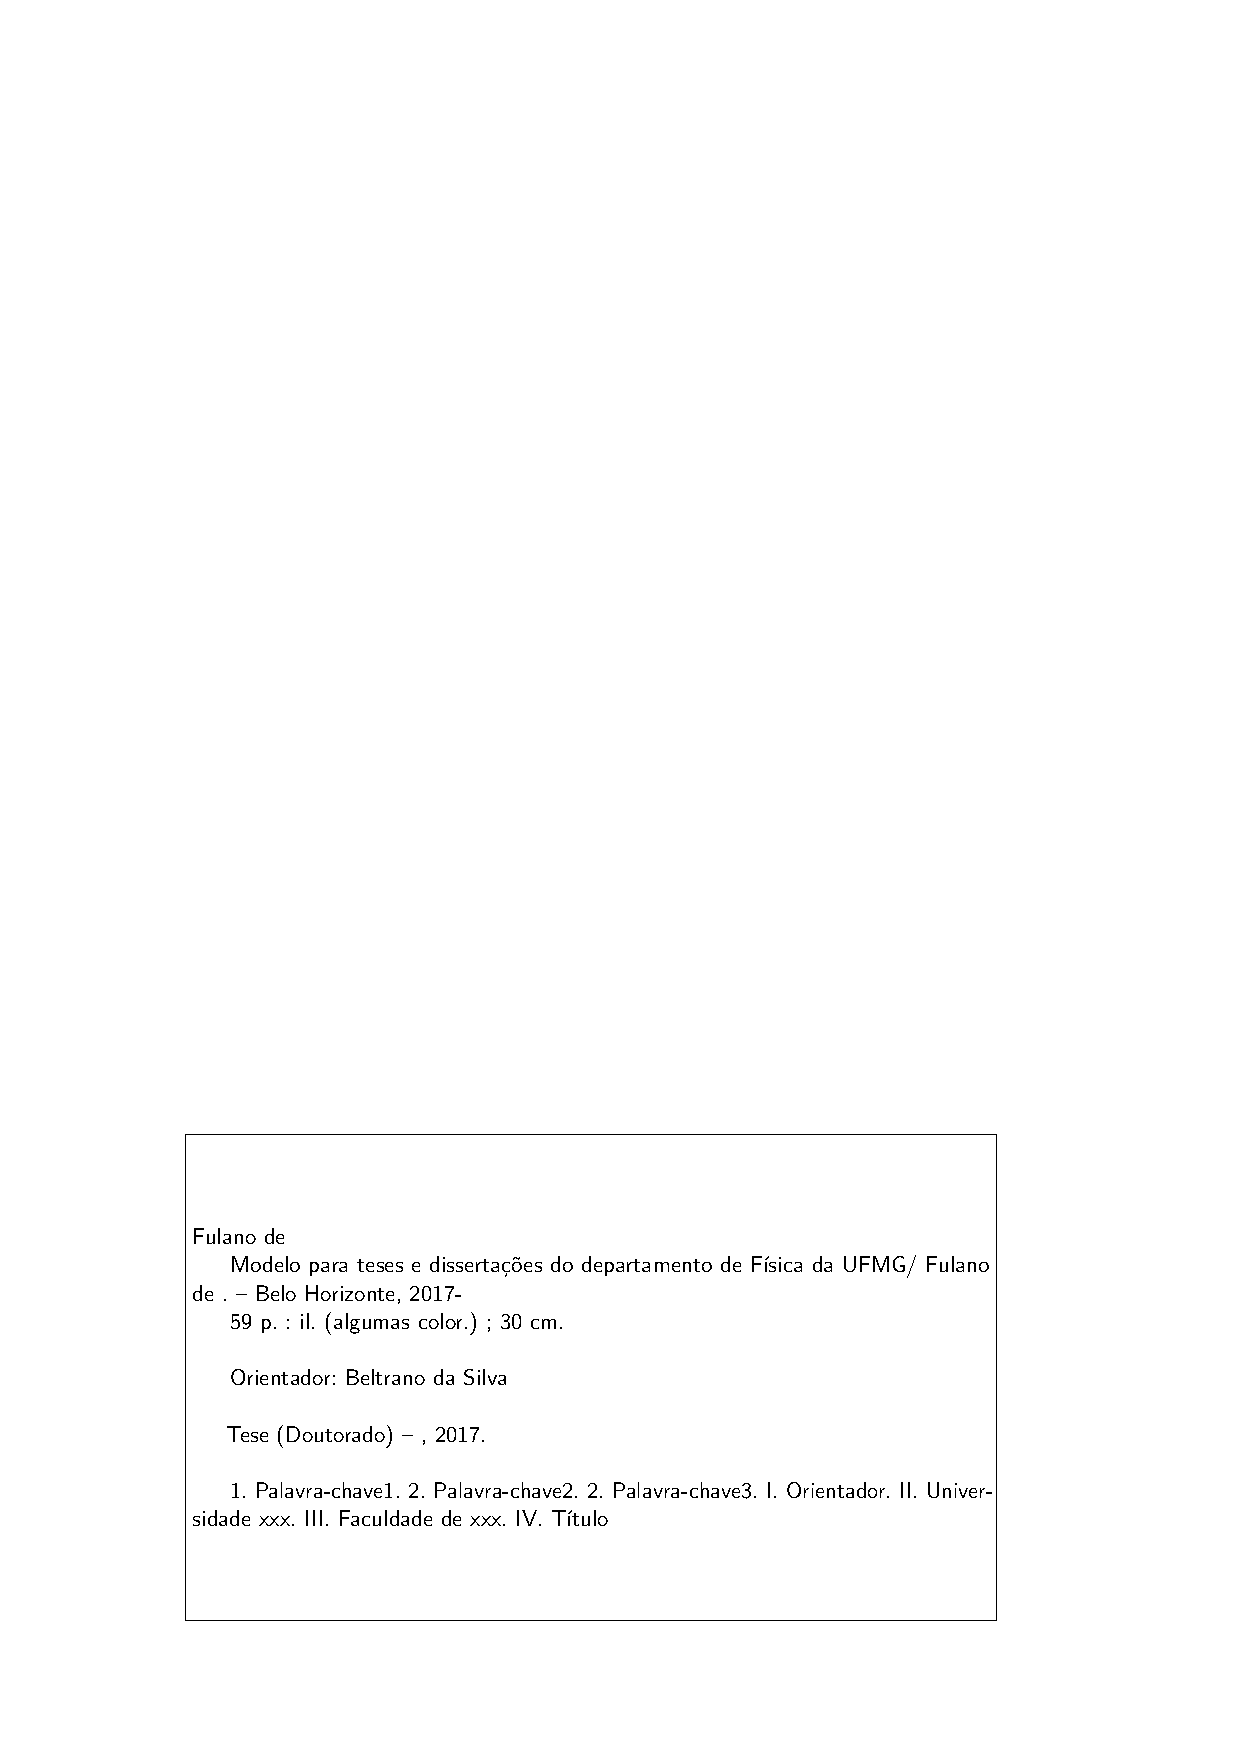
\includepdf{fig/ficha-catalografica.pdf}
\end{fichacatalografica}

% ---
% Inserir folha de aprovação
% ---

% A folha de aprovação é um elemento obrigatório da versão final do trabalho e deverá ser incluído
% conforme comando abaixo.
%
\begin{folhadeaprovacao}
     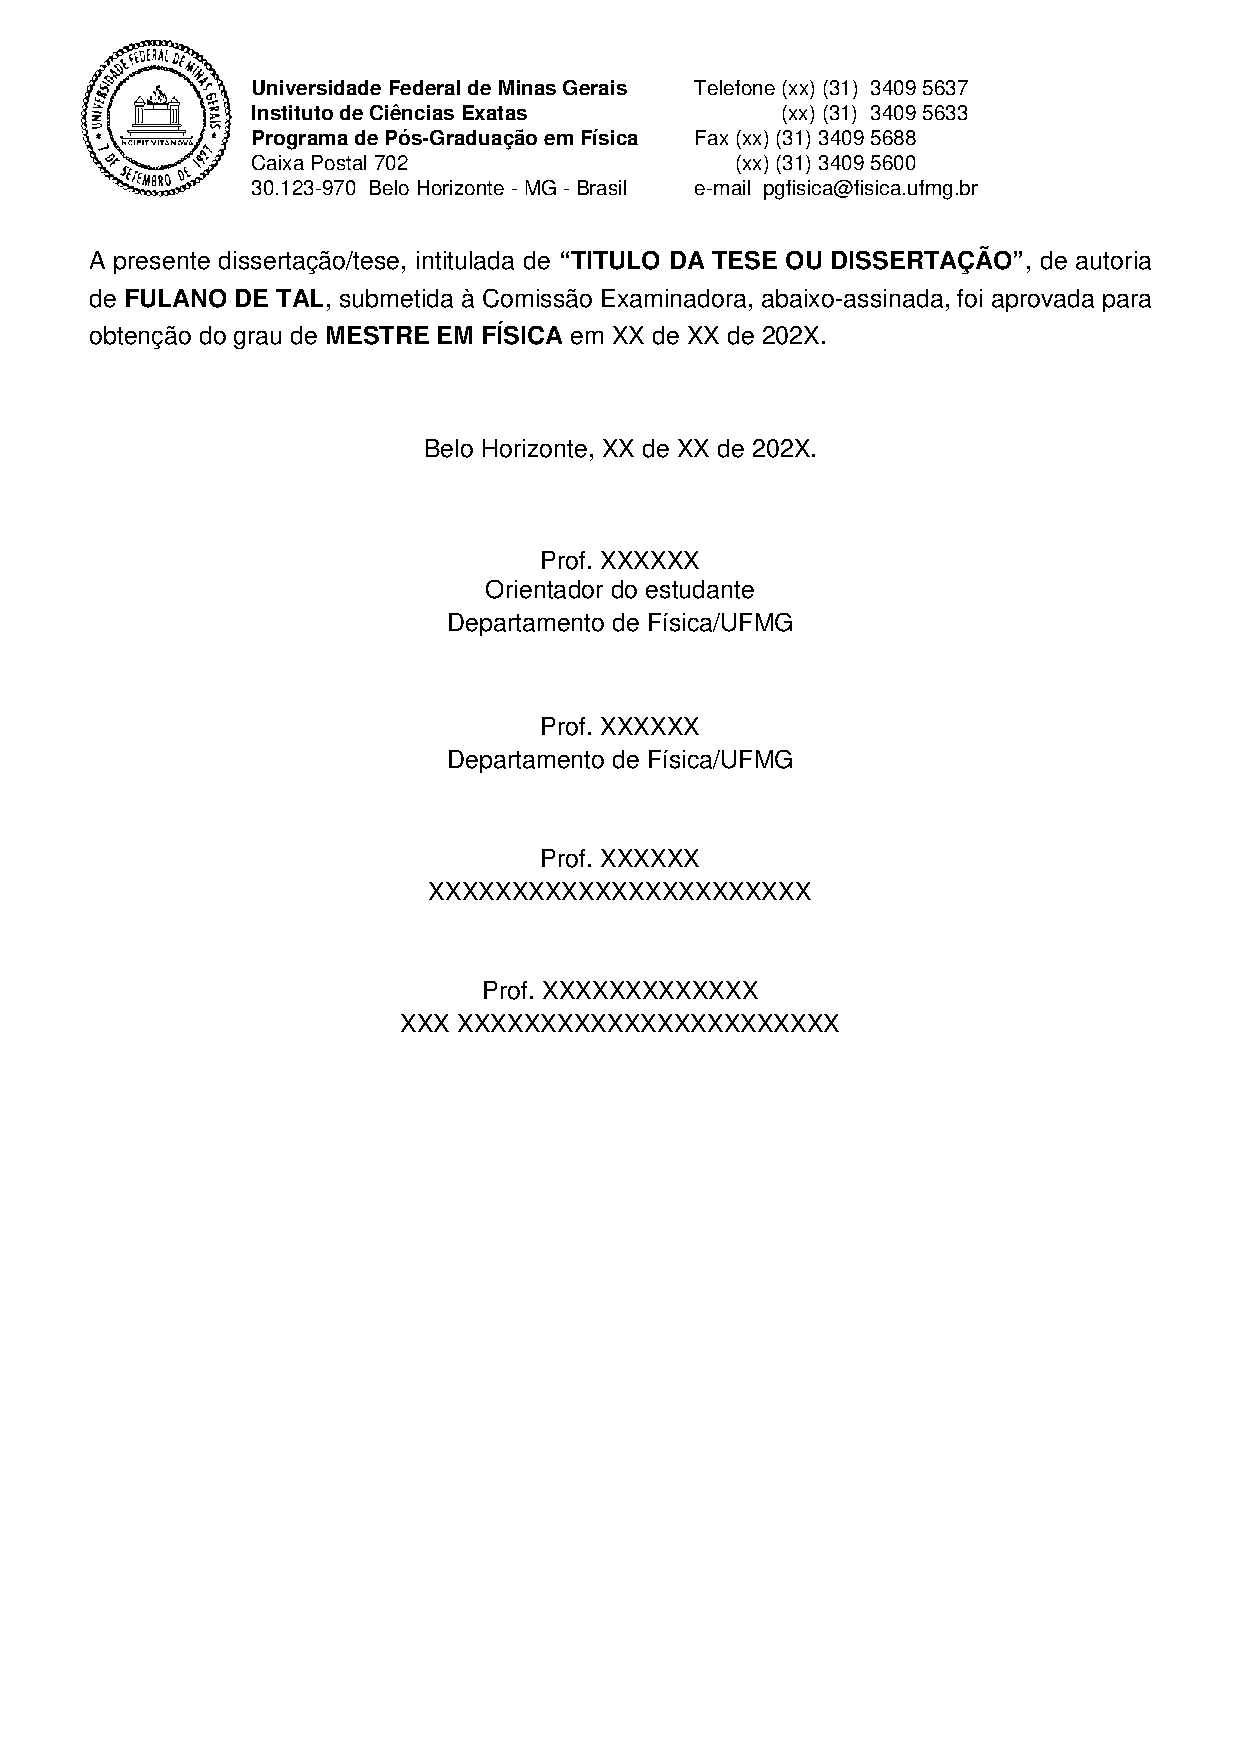
\includepdf{fig/folhadeaprovação.pdf}
     \end{folhadeaprovacao}
% ---
% Dedicatória - OPCIONAL
% ---
%\begin{dedicatoria}
%   \vspace*{\fill}
%   \centering
%   \noindent
%   \textit{\textbf{Dedicatória. Elemento opcional. Não há formatação a ser seguida.}\\
%    Este trabalho é dedicado às crianças adultas que,\\
%   quando pequenas, sonharam em se tornar cientistas.} \vspace*{\fill}
%\end{dedicatoria}
% ---

% ---
% Agradecimentos
% ---
\begin{agradecimentos}
Os agradecimentos são obrigatórios para os bolsistas e opcional para os demais. 
\end{agradecimentos}
% ---
% ---
% Epígrafe - OPCIONAL
% ---
%\begin{epigrafe}
%    \vspace*{\fill}
%	\begin{flushright}
%		\textit{\textbf{Epígrafe. Elemento opcional. Não há formatação a ser seguida.}\\
%		``Não vos amoldeis às estruturas deste mundo, \\
%		mas transformai-vos pela renovação da mente, \\
%		a fim de distinguir qual é a vontade de Deus: \\
%		o que é bom, o que Lhe é agradável, o que é perfeito.\\
%		(Bíblia Sagrada, Romanos 12, 2)}
%	\end{flushright}
%\end{epigrafe}
% ---

% ---
% RESUMOS
% ---

% resumo em português
\setlength{\absparsep}{18pt} % ajusta o espaçamento dos parágrafos do resumo
\begin{resumo}
O Resumo em português é um elemento obrigatório. Consiste de uma síntese de pontos relevantes com apresentação do objetivo, métodos, técnicas, resultados e conclusões. Deve apresentar, abaixo, as palavras-chave relacionadas ao trabalho. Não pode exceder uma página.

   \vspace{\onelineskip}
 
   \noindent 
 \textbf{Palavras-chave}: Modelo, Tese, Dissertação, Projeto

\end{resumo}

% resumo em inglês
\begin{resumo}[Abstract]
 \begin{otherlanguage*}{english}
The abstract and keywords, in English, are also mandatory and must fit in one page.
   \vspace{\onelineskip}
 
   \noindent 
   \textbf{Keywords}: Template, Dissertations, Thesis, Projects.
 \end{otherlanguage*}

\end{resumo}

% ---
% LISTAS - CONTEÚDO DE CARÁTER OPCIONAL
% ---
% ---
% AS LISTAS DE ILUSTRAÇÕES, TABELAS, ABREVIATURAS E SIGLAS E SÍMBOLOS SÃO ELEMENTOS OPCIONAIS.
% RESSALTA-SE A IMPORTÂNCIA DE SE AO UTILIZAR TAIS LISTAS INCLUIR CORRETAMENTE NO LATEX UM TÍTULO
% PARA CADA FIGURA OU TABELA AO INVÉS DE DEIXAR A LEGENDA COMPLETA, QUE É, EM GERAL, MUITO GRANDE
% E POUCO INSTRUTIVA. ISTO É FEITO COM O SEGUINTE COMANDO: \caption[título da figura]{Legenda da figura}
% ---

% ---
% inserir lista de ilustrações - OPCIONAL
% ---
%\pdfbookmark[0]{\listfigurename}{lof}
%\listoffigures*
%\cleardoublepage
% ---

% ---
% inserir lista de tabelas - OPCIONAL
% ---
%\pdfbookmark[0]{\listtablename}{lot}
%\listoftables*
%\cleardoublepage
% ---

% ---
% inserir lista de abreviaturas e siglas - OPCIONAL
% ---
%\begin{siglas}
%  \item[ABNT] Associação Brasileira de Normas Técnicas
%  \item[abnTeX] ABsurdas Normas para TeX
%\end{siglas}
% ---

% ---
% inserir lista de símbolos - OPCIONAL
% ---
%\begin{simbolos}
%  \item[$ \Gamma $] Letra grega Gama
%  \item[$ \Lambda $] Lambda
%  \item[$ \zeta $] Letra grega minúscula zeta
%  \item[$ \in $] Pertence
%\end{simbolos}
% ---



% ---
% O SUMARIO É OBRIGATÓRIO
% ---

% ---
% inserir o sumario
% ---
\pdfbookmark[0]{\contentsname}{toc}
\tableofcontents*
\cleardoublepage
% ---




% ----------------------------------------------------------
% ELEMENTOS TEXTUAIS
% ----------------------------------------------------------
\textual

\include{tex/cap1}

%\chapter{Introdução}

Este é o capítulo introdutório com exemplo de uma referência padrão \cite{exemplo}. \textbf{Ressalta-se que o texto: ``Citado na página ...'' é opcional e que outras formatações também podem ser usadas.}
 

\chapter{Comandos básicos do \LaTeX \label{cap1}}


Aqui apresentamos os comandos mais básicos para preparação de um trabalho em \LaTeX. Para mais detalhes sugere-se, por exemplo, ``The not so short introduction to  \LaTeX\  2$\varepsilon$''\cite{lshort}, que pode ser obtido em \url{http://tug.ctan.org/info/lshort/english/lshort.pdf} e o manual da classe \abnTeX\ \cite{abntex2classe} que foi a classe utilizada na confecção deste modelo. Perceba que há links no arquivo pdf que permitem clicar sobre o número da referência e ser enviado para lista de referências e que na última podem ser colocados links para os documentos referenciados.

Comentários em um arquivo \LaTeX\  podem ser introduzidos através do caracter \%. 

\section{Dicas gerais}

A principal dica que daremos neste texto é quanto ao \emph{Character Encoding} a ser usado nos arquivos. A classe \abnTeX, utilizada na confecção deste modelo, é baseada no \emph{encoding} UTF-8. Desta forma, recomenda-se fortemente que \textbf{todos} os arquivos sigam este padrão para não haver problemas com acentos, por exemplo. Isto pode ser facilmente configurado na grande maioria dos editores \LaTeX.

Outra dica importante ao usar o  \LaTeX\ na confecção de trabalhos longos é que se pode dividir o arquivo fonte em vários arquivos e usar os comandos \verb+\input{arquivo}+ e \verb+\include{arquivo}+. Esta estrutura foi adotada na confecção deste modelo. As diferenças entre os dois comandos é que no primeiro não são criados os arquivos auxiliares para o arquivo incluído e seu conteúdo não necessariamente se iniciam em uma nova página, enquanto no segundo arquivos auxiliares próprios são criados e o seu conteúdo se inicia em uma nova página. A recomendação é que pequenos trechos do trabalho sejam incluídos com o comando \verb+\input+ enquanto trechos maiores, como um capítulo, por exemplo, sejam incluídos através do comando \verb+\include+. Ao utilizar vários arquivos, apenas o arquivo fonte principal deve ser compilado. Recomenda-se o uso de editores   \LaTeX\ que permitam a criação de projetos, o que facilita ainda mais a navegação pelos vários arquivos, a compilação, visualização, etc. Alguns editores recomendados são:
TeXmaker (Linux, Mac, Windows), TeXstudio (Linux, Mac, Windows), TeXnicCenter (Windows), Kile (Linux). 

\section{Incluindo referências}

Uma das grandes vantagens no uso do \LaTeX\ na confecção de trabalhos acadêmicos é a facilidade de se incluir, numerar e gerenciar referências bibliográficas através de pacotes como o BibTeX. Desta forma, recomendamos o uso do último para gerenciar suas referências. A grande maioria dos editores de revistas científicas, assim como o google books e outros sites fornecem arquivos com os dados bibliográficos em formato BibTeX. Assim, basta criar um arquivo, com extensão \verb+.bib+, que contenha os dados das referências usadas e adicioná-lo ao arquivo fonte, em local apropriado, através do comando \verb+\bibliography{nome_do_arquivo.bib}+. É importante salientar que o uso correto do BibTeX depende de uma compilação inicial do arquivo fonte \LaTeX, seguida da compilação BibTeX e mais duas compilações   \LaTeX. Isto permite a criação da lista de referências e o correto ordenamento destas ao longo do texto e na seção de referências. De fato, o arquivo \verb+.bib+ pode conter muito mais referências que as efetivamente utilizadas no texto de forma que apenas as que forem citadas no texto serão incluídas na seção de referências. Além disso, a formatação que será dada à lista de referências, assim como as informações disponíveis no arquivo \verb+.bib+ que serão efetivamente utilizadas, são definidas pelo padrão adotado para as referências. Sugere-se que o formato a ser adotado seja o formato \verb+unsrt+ que foi selecionado neste documento através dos comandos:\\
\verb+\usepackage[fixlanguage]{babelbib}+\\
\verb+\selectbiblanguage{brazil}+\\
\verb+\bibliographystyle{babunsrt}+\\
em locais apropriados. Além disso, alguns dos editores recomendados anteriormente permitem o gerenciamento inclusive das referências ao se criar um projeto, o que facilita enormemente a inclusão de novas citações no texto.

Cada entrada do arquivo \verb+.bib+ tem estrutura similar à mostrada abaixo:
\begin{verbatim}
@article{exemplo,
	author={ R. M. Herman and A. Asgharian},
	journal={J. Mol. Spectrosc.},
	volume={19},
	pages={305},
	year={1966},
}
\end{verbatim}
Para fazer uma citação à esta referência basta incluir o comando \verb+\cite{exemplo}+, o que produz: \cite{exemplo}. A formatação dada a cada entrada depende do estilo selecionado. Para exemplificar, seguem citações a vários documentos que foram retiradas dos modelos do \abnTeX\ \cite{abntex2modelo}: \cite{guizzardi2005,macedo2005,EIA649B,masolo2010,guarino1995,bates2010,doxiadis1965}.
 \textbf{Ressalta-se que o texto: ``Citado na página ...'' presente na lista de referências é opcional e que outras formatações podem ser usadas.}

\newpage


\section{\label{estruturacao}Estruturação do texto}

Para iniciar este capítulo utilizamos o comando \\ \verb+\chapter{Comandos básicos do \LaTeX \label{cap1}}+.\\ O comando \verb+\label{cap1}+ é opcional e foi introduzido para permitir posteriores referências ao capítulo. Por exemplo, o comando \verb+\ref{cap1}+, produz o seguinte resultado: \ref{cap1}, e pode ser usado para fazer referências a este capítulo ao longo do texto. A numeração é automaticamente atualizada caso um novo capítulo seja introduzido. De fato, qualquer parte do texto, figuras, tabelas, equações, etc podem ser nomeadas pelo comando \verb+\label+ e posteriormente referenciadas pelo comando \verb+\ref+.

Seções dentro de um capítulo podem ser introduzidas pelo comando \\ \verb+\section{\label{estruturacao}Estruturação do texto}+. \\ Subseções são incluídas com o comando \verb+\subsection{Nome da subseção}+. Pode-se também usar \verb+\subsubsection+ e assim por diante. Caso o capítulo ou seção tenham um nome muito grande pode-se optar por introduzir um  nome resumido para o sumário e cabeçalho das páginas usando, por exemplo, \verb+\section[título resumido]{título longo}+.

\section{Equações, figuras e tabelas}

\subsection{Equações}

Equações podem ser inseridas através do ambiente \verb+equation+. Como exemplo, o comando:
\begin{verbatim}
\begin{equation}
\label{Z1}
Z=\sum_E g(E) e^{-\beta E}=e^{-\beta \epsilon_0}\sum_n g_n \left 
( e^{-\beta \epsilon}\right )^n=e^{-\beta \epsilon_0}\sum_n g_n z^n,
\end{equation}
\end{verbatim}
produz a seguinte equação:
\begin{equation}
\label{Z1}
Z=\sum_E g(E) e^{-\beta E}=e^{-\beta \epsilon_0}\sum_n g_n \left 
( e^{-\beta \epsilon}\right )^n=e^{-\beta \epsilon_0}\sum_n g_n z^n,
\end{equation}
Podemos, então, no texto introduzir facilmente referências à equação \ref{Z1} usando o comando \verb+\ref{Z1}+.

\subsection{Figuras}

Figuras podem ser introduzidas usando o comando, retirado da Ref.~\cite{abntex2classe}:
\begin{verbatim}
\begin{figure}[htb]
	\caption{\label{fig_grafico}Gráfico produzido em Excel e salvo como PDF}
	\begin{center}
	    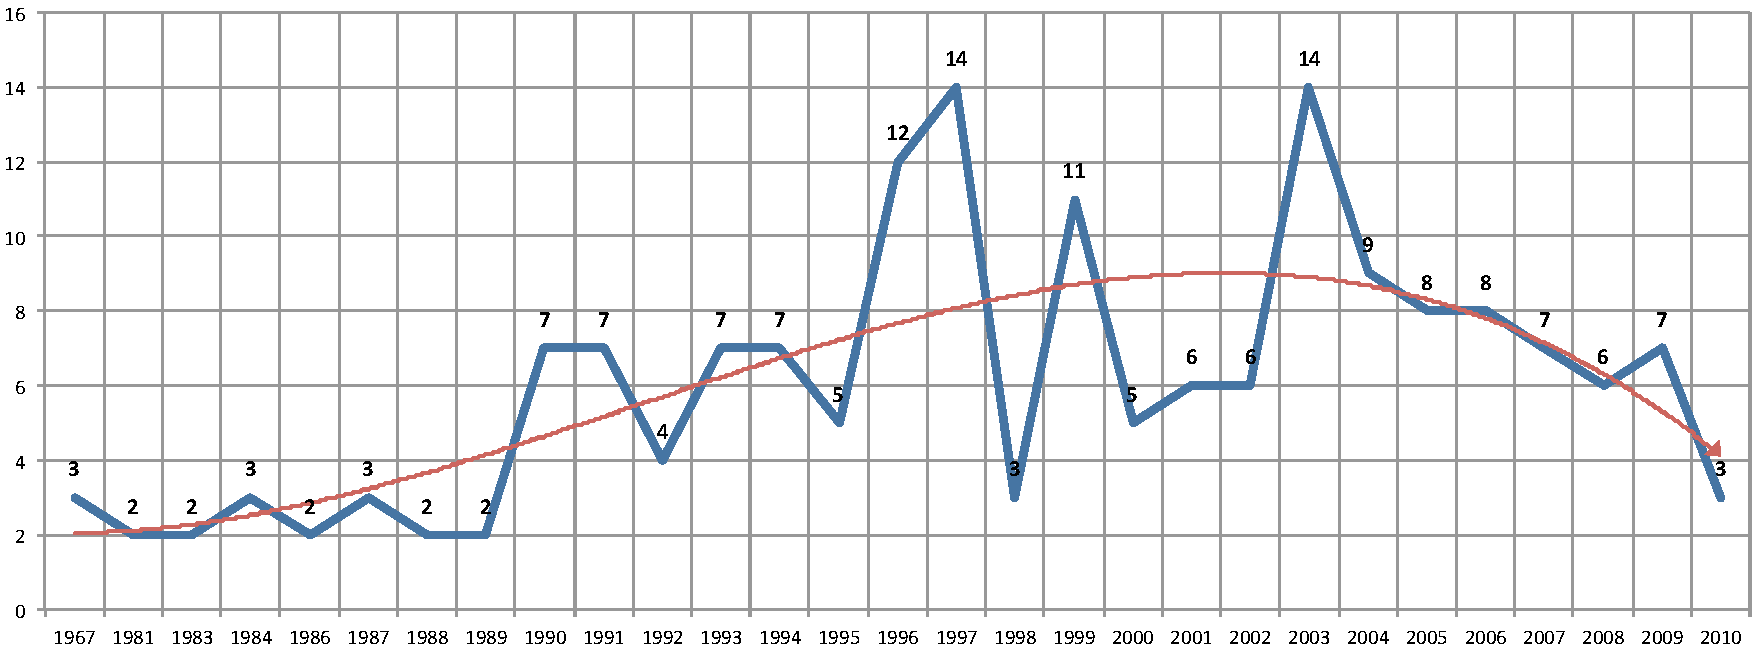
\includegraphics[scale=0.5]{fig/abntex2-modelo-img-grafico.pdf}
	\end{center}
	\legend{Fonte: \cite[p. 24]{araujo2012}}
\end{figure}
\end{verbatim}
Ressalta-se que ao invés de estabelecer a escala da figura através do comando \verb+scale=0.5+, poderia-se definir sua largura ou altura através de \verb+width+ ou \verb+height+ usando, por exemplo, \\ \verb+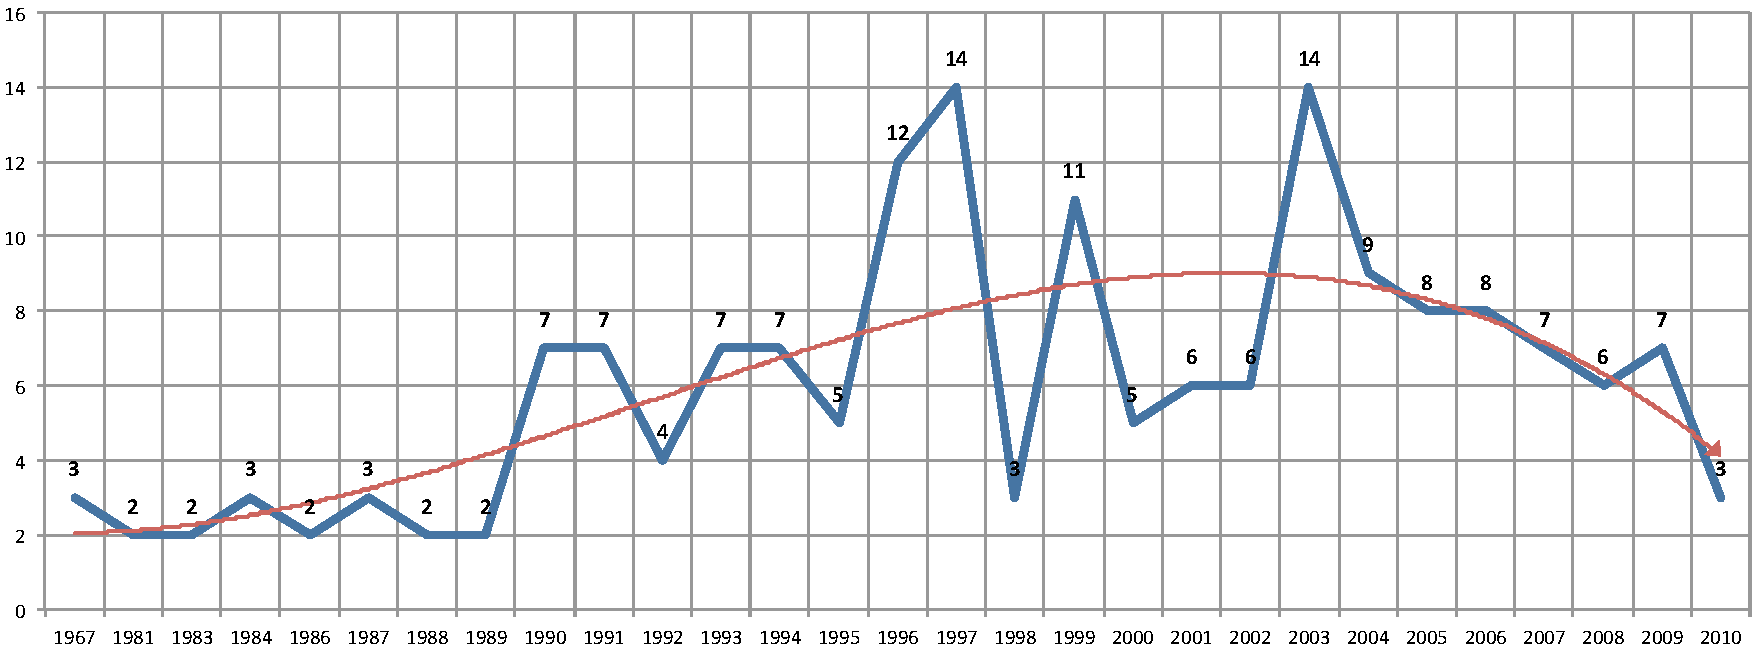
\includegraphics[width=5cm]{fig/abntex2-modelo-img-grafico.pdf}+ que re-escalaria a figura de forma a ela ficar com 5 cm de largura. Pode-se ainda usar \verb+0.5\linewidth+ ao invés de \verb+5cm+ para estabelecer a largura da figura como sendo metade da largura da linha do texto. O posicionamento da figura é definido pelo próprio \LaTeX. Recomenda-se colocar o comando o mais próximo possível do lugar onde a figura é citada. Por fim, recomenda-se usar figuras em formato \verb+pdf+.

\begin{figure}[htb]
	\caption{\label{fig_grafico}Gráfico produzido em Excel e salvo como PDF}
	\begin{center}
	    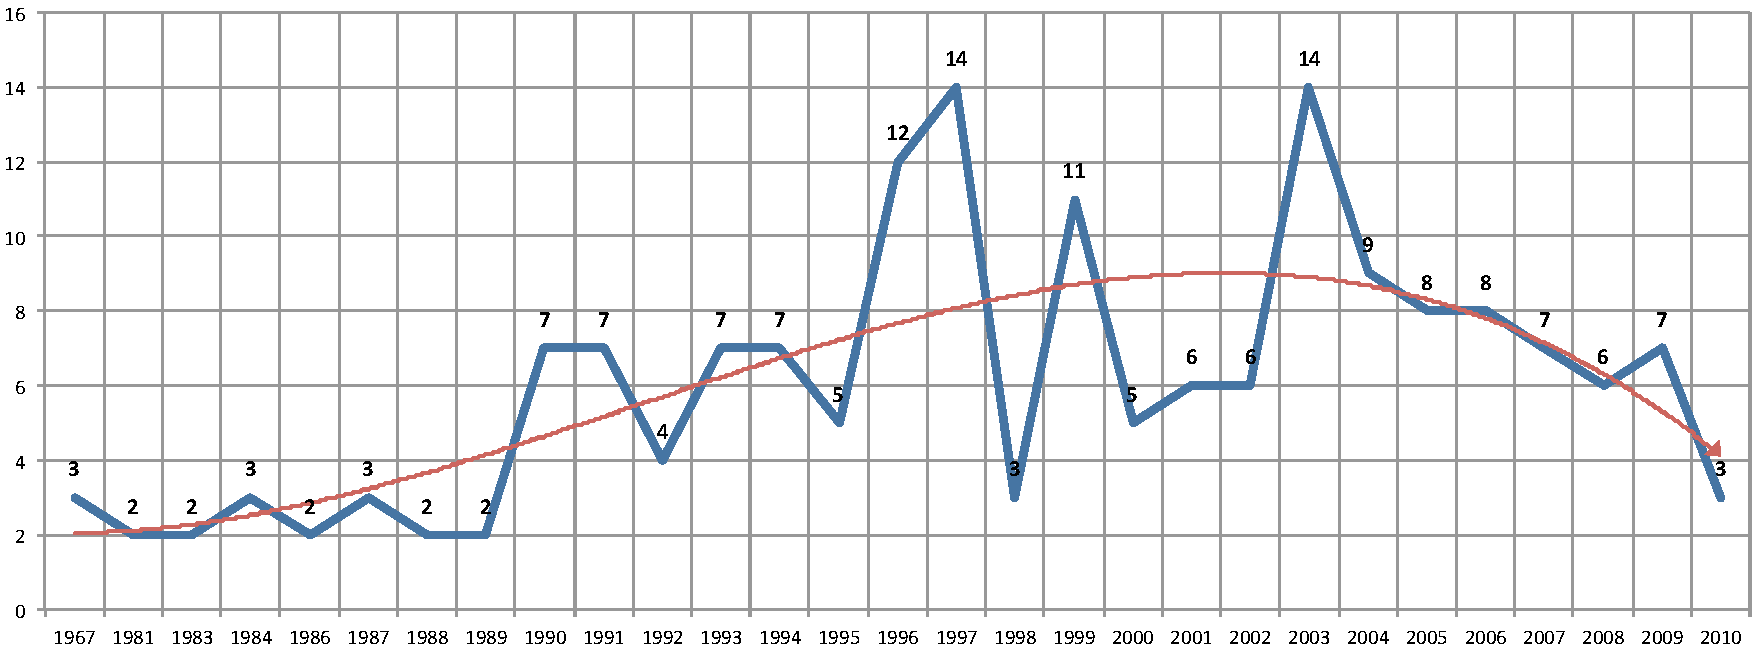
\includegraphics[scale=0.5]{fig/abntex2-modelo-img-grafico.pdf}
	\end{center}
	\legend{Fonte: \cite[p. 24]{araujo2012}}
\end{figure}


\subsection{Tabelas}

Há de se admitir que a confecção de tabelas em \LaTeX\ envolve uma prática um pouco maior. Abaixo apresentamos o comando que gerou a Tabela~\ref{tab1}. Uma dica interessante é que o comando \verb+\resizebox+ permite ajustar a tabela à largura do texto e é especialmente útil em situações onde a largura da tabela seria maior que a largura do texto.
\begin{scriptsize}
\begin{verbatim}
\begin{table}[ht] 
    \caption{Publicações relacionadas a alguma área em periódicos selecionados.
    \label{tab1}}
		\resizebox{\linewidth}{!}{%
\begin{tabular}{|l|c|c|c|c|c|c|c|c|c|}
    \hline
\multirow{2}{*}{\textbf{PERIÓDICO}} & \multicolumn{9}{c|}{ANOS}
\\ \cline{2-10}
& 2009&	2010&	2011&	2012&	2013&	2014&	2015& 2016& 2017\\ \hline
\textit{International Journal of Something} &	13&	15&	16&	15&	17&	17&	22& 22& 14\\ \hline 
\textit{Text Horizons}               		& 	6&	6&	9&	6&	8&	7&	19& 7& 6\\ \hline 
\textit{The Blablabla Review}             & 	8&	14&	9&	9&	15&	13&	21& 15& 9\\ \hline 
\textit{Journal of Magic}		&	2&	4&	2&	5&	1&	5&	1& 7& 4\\ \hline 
\textbf{TOTAL}&                           	29&	39&	36&	35&	41&	42&	63& 51& 33\\ \hline 
\multicolumn{8}{l}{Confeccionado pelo autor.}
\end{tabular}%
}
\end{table}
\end{verbatim}
\end{scriptsize}

\begin{table}[ht] 
    \caption{Publicações relacionadas a alguma área em periódicos selecionados.
    \label{tab1}}
		\resizebox{\linewidth}{!}{%
\begin{tabular}{|l|c|c|c|c|c|c|c|c|c|}
    \hline
\multirow{2}{*}{\textbf{PERIÓDICO}} & \multicolumn{9}{c|}{ANOS}
\\ \cline{2-10}
& 2009&	2010&	2011&	2012&	2013&	2014&	2015& 2016& 2017\\ \hline
\textit{International Journal of Something} &	13&	15&	16&	15&	17&	17&	22& 22& 14\\ \hline 
\textit{Text Horizons}               		& 	6&	6&	9&	6&	8&	7&	19& 7& 6\\ \hline 
\textit{The Blablabla Review}             & 	8&	14&	9&	9&	15&	13&	21& 15& 9\\ \hline 
\textit{Journal of Magic}		&	2&	4&	2&	5&	1&	5&	1& 7& 4\\ \hline 
\textbf{TOTAL}&                           	29&	39&	36&	35&	41&	42&	63& 51& 33\\ \hline 
\multicolumn{8}{l}{Confeccionado pelo autor.}
\end{tabular}%
}
\end{table}


\chapter{Conclusões}

Conclusões.




% ----------------------------------------------------------
% ELEMENTOS PÓS-TEXTUAIS
% ----------------------------------------------------------
\postextual
% ----------------------------------------------------------

% ----------------------------------------------------------
% Referências bibliográficas
% ----------------------------------------------------------
\bibliographystyle{babunsrt}
\bibliography{tex/references}

% ----------------------------------------------------------
% Glossário
% ----------------------------------------------------------
%
% Consulte o manual da classe abntex2 para orientações sobre o glossário.
%
%\glossary

% ----------------------------------------------------------
% Apêndices
% ----------------------------------------------------------

% ---
% Inicia os apêndices
% ---
\begin{apendicesenv}

% Imprime uma página indicando o início dos apêndices
\partapendices

% ----------------------------------------------------------
\chapter{Quisque libero justo}
% ----------------------------------------------------------

\lipsum[50]

% ----------------------------------------------------------
\chapter{Nullam elementum urna vel imperdiet sodales elit ipsum pharetra ligula
ac pretium ante justo a nulla curabitur tristique arcu eu metus}
% ----------------------------------------------------------
\lipsum[55-57]

\end{apendicesenv}
% ---


% ----------------------------------------------------------
% Anexos
% ----------------------------------------------------------

% ---
% Inicia os anexos
% ---
\begin{anexosenv}

% Imprime uma página indicando o início dos anexos
\partanexos

% ---
\chapter{Morbi ultrices rutrum lorem.}
% ---
\lipsum[30]

% ---
\chapter{Cras non urna sed feugiat cum sociis natoque penatibus et magnis dis
parturient montes nascetur ridiculus mus}
% ---

\lipsum[31]

% ---
\chapter{Fusce facilisis lacinia dui}
% ---

\lipsum[32]

\end{anexosenv}

%---------------------------------------------------------------------
% INDICE REMISSIVO - ELEMENTO OPCIONAL
%---------------------------------------------------------------------
%\phantompart
%\printindex
%---------------------------------------------------------------------


\end{document}
